\chapter{Discussion}
\label{cha:Discussion}
The following chapter discusses the results from the different approaches further and compares them to the 
results achieved by Micha Birklbauer in \cite[]{Birklbauer2021}. Additionally, possible future steps are discussed.
\section[]{Performance comparison}
Within this section the results of this thesis are compared to the results of \cite[]{Birklbauer2021} on a protein level.
\subsection[]{\acrfull*[]{ache}}
The following table represents the results for the \acrshort*[]{ache} protein in \cite[]{Birklbauer2021}:
\begin{figure}[H]
    \begin{center}
        \caption[]{Scoring results for ACHE Birklbauer}
        \label{fig:ache_birklbauer}
        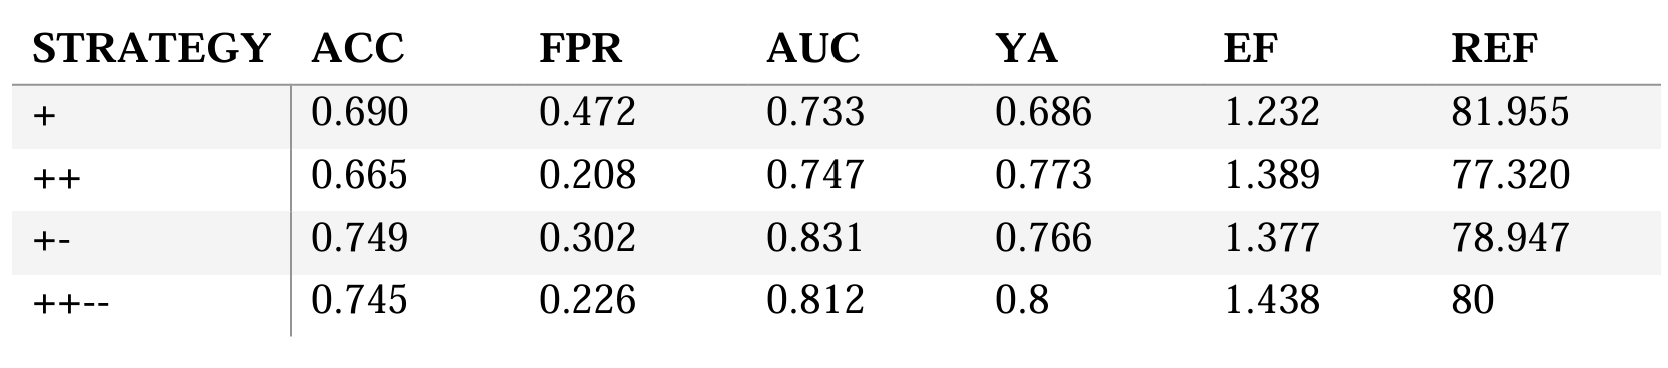
\includegraphics[width=14cm]{discussion/Birklbauer_ACHE.png}
    \end{center}
\end{figure}
The following results were achieved for the \acrshort*[]{ache} protein using the methods proposed in this thesis:
\begin{table}[H]
    \begin{center}
        \caption{Acetylcholinesterase performance test-set}
        \begin{tabular}{lrrrrrr}
            \toprule
            Name             & ACC    & FPR    & AUC    & YA     & EF     & REF     \\
            \midrule
            baseline\_rf     & 0.8106 & 0.3285 & 0.7992 & 0.7716 & 1.4161 & 92.6829 \\
            fe\_smote\_rf    & 0.8007 & 0.3358 & 0.7894 & 0.7653 & 1.4046 & 91.4634 \\
            fe\_smote\_nn    & 0.7708 & 0.2993 & 0.7650 & 0.7684 & 1.4102 & 82.9268 \\
            baseline\_nn     & 0.7674 & 0.2920 & 0.7626 & 0.7701 & 1.4134 & 81.7073 \\
            fe\_rf\_per\_knn & 0.7575 & 0.4307 & 0.7420 & 0.7177 & 1.3172 & 91.4634 \\
            baseline\_knn    & 0.6844 & 0.5766 & 0.6629 & 0.6520 & 1.1966 & 90.2439 \\
            fe\_rf\_mdi\_knn & 0.5515 & 0.4307 & 0.5530 & 0.5986 & 1.0987 & 59.8639 \\
            \bottomrule
        \end{tabular}
    \end{center}
\end{table}

The comparison between the two tables underlines the performance improvements of the machine learning approaches
over the simple scoring functions introduced in \cite[]{Birklbauer2021}.
Generally the improvements in \acrshort*[]{acc} and \acrshort*[]{ref} are most notable.
The improvements in the \acrshort*[]{ref} metric are of particular interest, as there is less money spent on investigating false positive compounds.


\subsection[]{\acrfull*[]{cox1}}
The following table represents the results for the \acrshort*[]{cox1} protein in \cite[]{Birklbauer2021}:

\begin{figure}[H]
    \begin{center}
        \caption[]{Scoring results for \acrshort*[]{cox1} Birklbauer}
        \label{fig:cox1_birklbauer}
        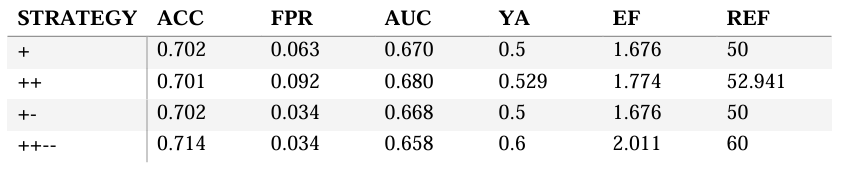
\includegraphics[width=14cm]{discussion/Birklbauer_COX1.png}
    \end{center}
\end{figure}

The results presented in the following table are the direct result of the methods proposed in this thesis:

\begin{table}[H]
    \begin{center}
        \caption{Cyclooxygenase 1 performance test-set}
        \begin{tabular}{lrrrrrr}
            \toprule
            Name             & ACC    & FPR    & AUC    & YA     & EF     & REF     \\
            \midrule
            baseline\_rf     & 0.7724 & 0.0183 & 0.6344 & 0.8710 & 2.8909 & 87.0968 \\
            fe\_smote\_rf    & 0.7628 & 0.0138 & 0.6155 & 0.8846 & 2.9362 & 88.4615 \\
            fe\_rf\_per\_knn & 0.7019 & 0.0826 & 0.5598 & 0.5135 & 1.7044 & 51.3514 \\
            baseline\_knn    & 0.6859 & 0.1147 & 0.5544 & 0.4565 & 1.5153 & 45.6522 \\
            baseline\_nn     & 0.6827 & 0.0872 & 0.5309 & 0.4242 & 1.4081 & 42.4242 \\
            fe\_smote\_nn    & 0.6827 & 0.1147 & 0.5490 & 0.4444 & 1.4752 & 44.4444 \\
            fe\_rf\_mdi\_knn & 0.6250 & 0.1835 & 0.4987 & 0.2982 & 0.9899 & 29.8246 \\
            \bottomrule
        \end{tabular}
    \end{center}
\end{table}
The machine learning algorithms were able to achieve higher accuracy scores while also improving on the \acrshort*[]{fpr} and the two enrichment factors. 
This means that the machine learning algorithms are more capable to correctly identify active and inactive protein-ligand complexes.

\subsection[]{\acrfull*[]{dpp4}}
The results for \acrshort*[]{dpp4} mentioned in \cite[]{Birklbauer2021} are presented below:
\begin{figure}[H]
    \begin{center}
        \caption[]{Scoring results for \acrshort*[]{dpp4} Birklbauer}
        \label{fig:dpp4_birklbauer}
        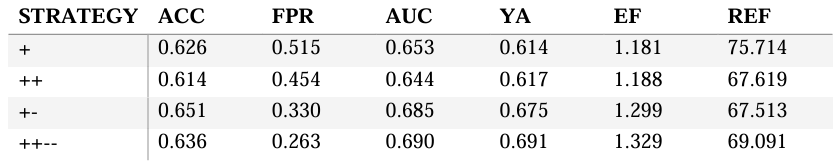
\includegraphics[width=14cm]{discussion/Birklbauer_DPP4.png}
    \end{center}
\end{figure}

The approaches documented within this thesis were able to achieve the following scores:
\begin{table}[H]
    \begin{center}
        \caption{Dipeptidyl peptidase IV performance test-set}
        \begin{tabular}{lrrrrrr}
            \toprule
            Name             & ACC    & FPR    & AUC    & YA     & EF     & REF     \\
            \midrule
            baseline\_rf     & 0.7721 & 0.2041 & 0.7730 & 0.7984 & 1.5393 & 79.8387 \\
            fe\_smote\_rf    & 0.7662 & 0.2122 & 0.7670 & 0.7912 & 1.5254 & 79.1165 \\
            fe\_rf\_per\_knn & 0.7112 & 0.3714 & 0.7082 & 0.6957 & 1.3412 & 78.7879 \\
            baseline\_nn     & 0.6896 & 0.3347 & 0.6887 & 0.6963 & 1.3425 & 71.2121 \\
            baseline\_knn    & 0.6896 & 0.3959 & 0.6865 & 0.6767 & 1.3046 & 76.8939 \\
            fe\_smote\_nn    & 0.6896 & 0.3306 & 0.6889 & 0.6978 & 1.3453 & 70.8333 \\
            fe\_rf\_mdi\_knn & 0.4892 & 0.5143 & 0.4891 & 0.5078 & 0.9791 & 50.7812 \\
            \bottomrule
        \end{tabular}
    \end{center}
\end{table}
The results for this protein differ drastically; The machine learning algorithms achieved 15\% better accuracy for the \acrshort*[]{dpp4} data. The values of the other metrics also improved when using the machine learning approaches.


\subsection[]{\acrfull*[]{maob}}
The following results were achieved for the \acrshort*[]{maob} protein in \cite[]{Birklbauer2021}:
\begin{figure}[H]
    \begin{center}
        \caption[]{Scoring results for \acrshort*[]{maob} Birklbauer}
        \label{fig:moab_birklbauer}
        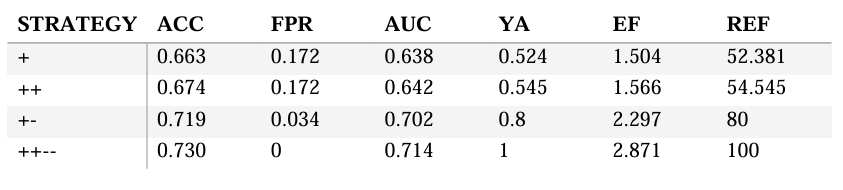
\includegraphics[width=14cm]{discussion/Birklbauer_MAOB.png}
    \end{center}
\end{figure}
The following table represents the results computed by the various machine learning algorithms proposed in this thesis:
\begin{table}[H]
    \begin{center}
        \caption{Monoamine oxidase B performance test-set}
        \begin{tabular}{lrrrrrr}
            \toprule
            Name             & ACC    & FPR    & AUC    & YA     & EF     & REF     \\
            \midrule
            baseline\_rf     & 0.7589 & 0.1389 & 0.7181 & 0.6970 & 1.9515 & 69.6970 \\
            fe\_rf\_per\_knn & 0.7054 & 0.1944 & 0.6653 & 0.6000 & 1.6800 & 60.0000 \\
            fe\_smote\_rf    & 0.7054 & 0.1944 & 0.6653 & 0.6000 & 1.6800 & 60.0000 \\
            baseline\_nn     & 0.6964 & 0.1806 & 0.6472 & 0.5938 & 1.6625 & 59.3750 \\
            baseline\_knn    & 0.6786 & 0.1667 & 0.6167 & 0.5714 & 1.6000 & 57.1429 \\
            fe\_smote\_nn    & 0.6696 & 0.2222 & 0.6264 & 0.5429 & 1.5200 & 54.2857 \\
            fe\_rf\_mdi\_knn & 0.5804 & 0.3333 & 0.5458 & 0.4146 & 1.1610 & 42.5000 \\
            \bottomrule
        \end{tabular}
    \end{center}
\end{table}
While the accuracy of the top performing machine learning algorithm is better than all the results in \cite[]{Birklbauer2021} for \acrshort*[]{maob}, the \acrshort*[]{fpr} and all the other metrics are higher for the \textit{++--} strategy in \cite[]{Birklbauer2021}.
\subsection[]{Soluble epoxide hydrolase}
The following table represents the results of the approaches implemented in \cite[]{Birklbauer2021} for soluble epoxide hydrolase:
\begin{figure}[H]
    \begin{center}
        \caption[]{Scoring results for soluble epoxide hydrolase Birklbauer}
        \label{fig:seh_birklbauer}
        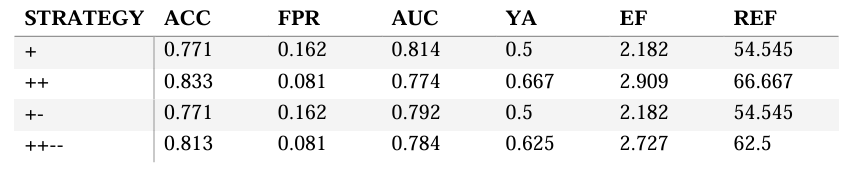
\includegraphics[width=14cm]{discussion/Birklbauer_SEH.png}
    \end{center}
\end{figure}
The following results were achieved using the methods described within this thesis:
\begin{table}[H]
    \begin{center}
        \caption{Soluble epoxide hydrolase performance test-set}
        \begin{tabular}{lrrrrrr}
            \toprule
            Name             & ACC    & FPR    & AUC    & YA     & EF     & REF      \\
            \midrule
            fe\_rf\_per\_knn & 0.8000 & 0.0667 & 0.6667 & 0.6667 & 2.6667 & 66.6667  \\
            baseline\_nn     & 0.7833 & 0.0667 & 0.6333 & 0.6250 & 2.5000 & 62.5000  \\
            baseline\_rf     & 0.7667 & 0.0000 & 0.5333 & 1.0000 & 4.0000 & 100.0000 \\
            fe\_smote\_rf    & 0.7667 & 0.0000 & 0.5333 & 1.0000 & 4.0000 & 100.0000 \\
            baseline\_knn    & 0.7333 & 0.0222 & 0.4889 & 0.0000 & 0.0000 & 0.0000   \\
            fe\_rf\_mdi\_knn & 0.7000 & 0.1333 & 0.5333 & 0.3333 & 1.3333 & 33.3333  \\
            fe\_smote\_nn    & 0.7000 & 0.0889 & 0.4889 & 0.2000 & 0.8000 & 20.0000  \\
            \bottomrule
        \end{tabular}
    \end{center}
\end{table}
The accuracy performance in \cite[]{Birklbauer2021} is slightly better than the accuracy the machine learning algorithms where able to achieve. Still, the random forest methods where able to achieve better metrics overall.
The \acrshort*[]{fpr} and \acrshort*[]{ref} are particularly notable, as they represent the ideal values for drug discovery.

\section{Improvements and outlook}
This thesis serves as a proof of concept for the applicability of machine learning models in combination with feature engineering for protein docking, as the achieved results 
are more accurate than those achieved using traditional approaches.

However, the machine learning approaches for protein docking where implemented using standard approaches and models. 
Through the use of more problem-tailored algorithmic methods the quality of the results will probably increase. Additionally, only a small sample 
of protein-ligand complexes was researched for this thesis. The machine learning methods proposed within this thesis need to be evaluated on a larger subset of 
protein-ligand compounds to determine whether machine learning is a viable approach for protein docking.
